\documentclass[a4paper]{article}
\usepackage[utf8]{inputenc}
\usepackage{geometry}
\usepackage{polski}
\usepackage{graphicx}
\usepackage{float}
\usepackage{etoolbox,refcount}
\usepackage{multicol}

\newgeometry{left=2cm, right=2cm, bottom=1.5cm, top=1.5cm}

\begin{document}
	\begin{figure}[H]
		\centering
		\includegraphics[height=6cm, width=\textwidth]{./img/formatka.png}
	\end{figure}
	\section{Cel ćwiczenia}
		Celem ćwiczenia jest zapoznanie się z bezpośrednim sterowaniem cyfrowym z wykorzystaniem komputera z kartą przemysłową PCL 812, przy użyciu pakietu MATLAB/SIMULINK
	\section{Wstęp teoretyczny}
		Uproszczony schemat budowy stanowiska:
		\begin{figure}[H]
			\centering
			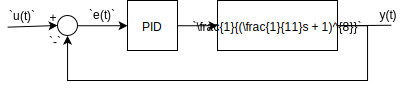
\includegraphics[width=\textwidth]{./img/schemat.png}
		\end{figure} 
		W tym ćwiczeniu używaliśmy trzech układów sterowania:
		\begin{itemize}
			\item algorytm PID
			\item układ regulacji dwupołożeniowej
			\item predyktor Smitha
		\end{itemize}
		\subsection{Algorytm PID}
			Jest to układ z pętlą sprzężenia zwrotnego, który realizuję akcję całkującą, różniczkującą i proporcjonalną. Jego transmitancja jest zadana wzorem:
			$$
				G(s) = K_p + \frac{K_p}{T_is} + T_d K_p s
			$$
			Regulator PID działa w pętli sprzężenia zwrotnego, dążąc do eliminacji uchybu, który jest wyliczany jako różnica pomiędzy wartością zadaną i zmierzoną wartością zmiennej procesu. Jest to najczęściej stosowana metoda regulacji ze wszystkich używanych w automatyce. 
			\begin{figure}[H]
				\centering
				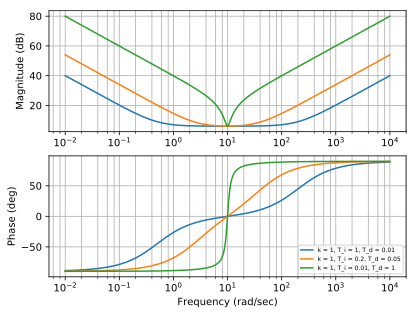
\includegraphics[width=0.6\textwidth]{./img/PID.png}
			\end{figure} 
		\subsection{Układ regulacji dwupołożeniowej}
			Układ regulacji dwupołożeniowej jest wykorzystywany w zadaniach, które nie wymagają zbyt dużej precyzji. Działa przełączając pomiędzy dwiema wartościami na wyjściu w zależności od stanu, jaki znajduje się na jego wejściu. Jest to bardzo tani system regulacji, którego głównym celem jest utrzymywanie wartości na wyjściu w pewnym przedziale. Często takie układy posiadają histerezę, aby nie wymuszać ich ciągłego przełączania. 
		\subsection{Predyktor Smitha}
			Predyktor Smitha jest układem używanym w przypadku układów z opóźnieniem, które jest nam znane. Układ ten zawiera dwie pętle sprzężenia zwrotnego, z których jedna jest normalną pętlą sprzężenia zwrotnego, a druga odpowiada za predykcję wyjścia układu.
	\section{Wykonanie ćwiczenia}
		Wykonanie ćwiczenia nie sprawiło nam problemu, jedyne problemy wystąpiły przy modelu z predyktorem Smitha, gdzie zapomnieliśmy ustawić parametr opóźnienia.
		\subsection{Algorytm PID}
			Schemat:
			\begin{figure}[H]
				\centering
				\includegraphics[width=\textwidth]{./img/PID_alg.png}
			\end{figure}
			\newpage
			Uchyb:
			\begin{figure}[H]
				\centering
				\includegraphics[width=\textwidth]{./img/PID_error.png}
			\end{figure}
		\subsection{Układ regulacji dwupołożeniowej}
			Schemat:
			\begin{figure}[H]
				\centering
				\includegraphics[width=\textwidth]{./img/relay_algo.png}
			\end{figure}
			\newpage
			Wyjście:
			\begin{figure}[H]
				\centering
				\includegraphics[width=\textwidth]{./img/relay_out.png}
			\end{figure}
		\subsection{Predyktor Smitha}
			Schemat:
			\begin{figure}[H]
				\centering
				\includegraphics[width=\textwidth]{./img/smith_algo.png}
			\end{figure}
			\newpage
			Uchyb:
			\begin{figure}[H]
				\centering
				\includegraphics[width=\textwidth]{./img/smith_error.png}
			\end{figure}
		\subsection{Obserwacje}
			Na układzie można zobaczyć opóźnienie jakie jest generowane przez układ z jakim mamy do czynienia. Jest ono równe 30 sekund, co można odczytać na każdym z wykresów. W przypadku braku opóźnienia mielibyśmy do czynienia z efektywniejszym działaniem algorytmu PID oraz z zatrzymaniem się sterowania w układzie dwupołożeniowym w chwili gdy zadana wartość zostanie otrzymana. Można na podstawie tego opóźnienia uznać stosowanie predyktora Smitha za stosowne i uzasadnione. Ze względu na to, że nie mając czasu na przygotowanie się do ćwiczenia przeoczyliśmy fragment instrukcji odnośnie ustawienia opóźnienia w predyktorze Smitha na 18 sekund postanowiliśmy przy najbliższej możliwości naprawić ten błąd przeprowadzając symulację obiektu przy założeniu, że jego transmitancja jest zadana wzorem (dane zgodne ze specyfikacją zadania oraz tabelką zamieszczoną w dodatku):
			$$
				G(s) = e^{-18s} \cdot \frac{1.07}{1+43.8253\cdot s}
			$$
	\section{Obliczenia teoretyczne}
		Obliczenia te dokonaliśmy przy założeniu, że obiekt jest w pełni liniowy oraz, że opóźnienie wynosi tyle ile udało nam się odczytać z wykresu. Dodatkowo udało nam się wychwycić różnice pomiędzy modelem matematycznym w przypadku sterowania regulatorem dwupołożeniowym. Obiekt sterowania został zastąpiony następującym układem:
		\begin{figure}[H]
			\centering
			\includegraphics[width=0.5\textwidth]{./img/obiekt.png}
		\end{figure}
		\subsection{Algorytm PID}
			\begin{figure}[H]
				\centering
				\caption{Charakterystyka skokowa}
				\includegraphics[width=0.8\textwidth]{./img/PID_step.png}
			\end{figure}
			\begin{figure}[H]
				\centering
				\caption{Uchyb}
				\includegraphics[width=0.8\textwidth]{./img/PID_error_correct.png}
			\end{figure}
		\subsection{Regulator dwupołożeniowy}
			\begin{figure}[H]
				\centering
				\caption{Charakterystyka skokowa}
				\includegraphics[width=0.8\textwidth]{./img/dwapol_step.png}
			\end{figure}
			\begin{figure}[H]
				\centering
				\caption{Uchyb}
				\includegraphics[width=0.8\textwidth]{./img/dwapol_error.png}
			\end{figure}
		\subsection{Predyktor Smitha}
			\begin{figure}[H]
				\centering
				\caption{Charakterystyka skokowa}
				\includegraphics[width=0.8\textwidth]{./img/smith_step.png}
			\end{figure}
			\begin{figure}[H]
				\centering
				\caption{Uchyb}
				\includegraphics[width=0.8\textwidth]{./img/smith_error_correct.png}
			\end{figure}
	\section{Wnioski}
		Na podstawie przebiegów i wartości odczytanych z wykresu możemy wywnioskować, że doświadczenie odbywało się w innych warunkach niż omówione we wprowadzeniu. Wartość opóźnienia zgodnie z warunkami zadania powinna była wynosić 18 sekund, co jest prawdziwe, ale pod warunkiem, że mamy do czynienia z drugim wyjściem obiektu. Jednak opóźnienie generowane przez układ pozwala na stwierdzenie, że jest on najprawdopodobniej podpięty do złego wyjścia. Przeszkadza to tylko w wykonaniu części laboratorium odpowiedzialnej za wyznaczenie odpowiedzi układu z predyktorem Smitha. Obliczenia teoretyczne zostały już wykonane dla w pełni poprawnego zestawu danych zgodnego z tabelką zamieszczoną we wprowadzeniu do laboratorium. Ćwiczenie to pozwoliło nam na zapoznanie się z różnymi metodami bezpośredniego sterowania cyfrowego przy pomocy komputera, jak i nauczyło nas o dbałość o szczegóły. Zapoznaliśmy się z podstawowymi metodami predykcji w automatyce oraz z praktycznym zastosowaniem regulatora PID, jak i regulatora dwupołożeniowego.
		\newline 
		\newline
		Bazując na wykresach uzyskanych z symulacji w środowisku MATLAB/SIMULINK można zauważyć, że układ z predyktorem Smitha radzi sobie lepiej, gdyż jest mniej podatny na opóźnienia w przesyle informacji, jakie są generowane przez obiekt. Dodatkowo można zauważyć dosyć spore różnice pomiędzy wyliczeniami dla regulatora dwupołożeniowego oraz danymi zebranymi w trakcie wykonywania pomiarów.
		\newline 
		\newline
		Pogłębieniu uległa również nasza widza na temat środowiska MATLAB/SIMULINK, gdyż dowiedzieliśmy się o możliwości tworzenia własnych bloczków, które mogą komunikować się z innymi urządzeniami i pobierać z nich dane. Do tej pory były to dla nas tylko i wyłącznie narzędzia służące do przeprowadzenia symulacji z dziedziny automatyki i do szybkiej obróbki danych, które znajdowały się już na komputerze.
		\newline
		\newline
		Dowiedzieliśmy się również jak ważne może być modelowanie układów oraz jak dokładnym przybliżeniem rzeczywistości jest układ liniowy, porównując wyniki uzyskane z bezpośredniego pomiaru oraz te z symulacji przeprowadzonej na potrzeby poprawnego wykonania ćwiczenia. 
		\newline
		\newline 
		Ćwiczenie zostało wykonane w pełni, w zakresie jaki został nam zlecony przez prowadzącego, wykraczając nieznacznie poza zakres materiału, który powinien był zostać pokryty. Jednak było to konieczne aby uzupełnić nasze pomiary o wartości z predyktora Smitha.
\end{document}